\section{レポート課題 2nd}
\subsection{課題1}
\subsubsection{問題}
$r = 3.8285$ として、$x_n$ が$250 \leq n \leq 500$ の場合の時系列とリターンマップを描け、初期値は適当でよい。周期3を確認せよ(3周期の窓)
\subsubsection{画像}
\begin{figure}[htbp]
  \centering
  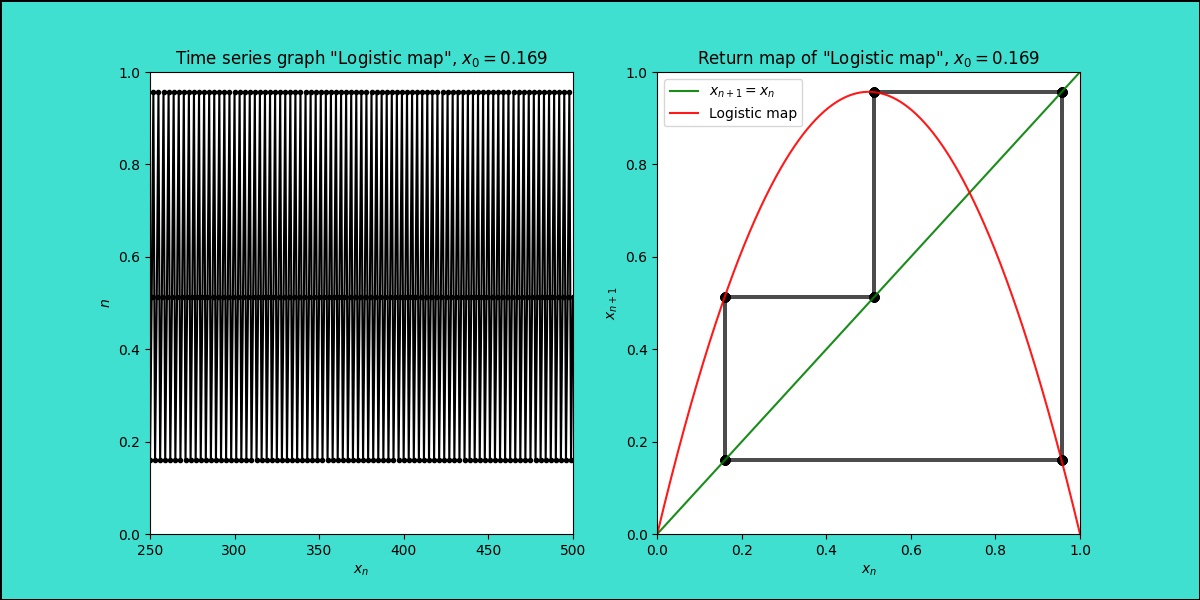
\includegraphics[keepaspectratio, scale=0.5]{images/Problem7/task7_1.png}
\end{figure}
\subsubsection{考察}
$r = 3.8285$ のときは、前回のレポート課題3に書いてあるロジスティック写像の分岐図を見ると、3周期解になっている範囲だとわかる。実際にグラフを描くと、時系列グラフ、リターンマップともに3つの解で周期性を持っていることが読み取れた。また、初期値をランダムにとって複数回プログラムを実行してもどちらのグラフにも変化は見られなかった。よって、$r = 3.8285$ のときはカオスの条件には当てはまらず周期性(3周期)を持っていると考察した。

\newpage
\subsection{課題2}
\subsubsection{問題}
$r = 3.8284$ として、$x_n$ が$250 \leq n \leq 500$ の場合の時系列とリターンマップを描け、初期値は適当でよい。規則的な部分(ラミナー)と不規則の部分(バースト)を確認せよ。
\subsubsection{画像}
\begin{figure}[htbp]
  \centering
  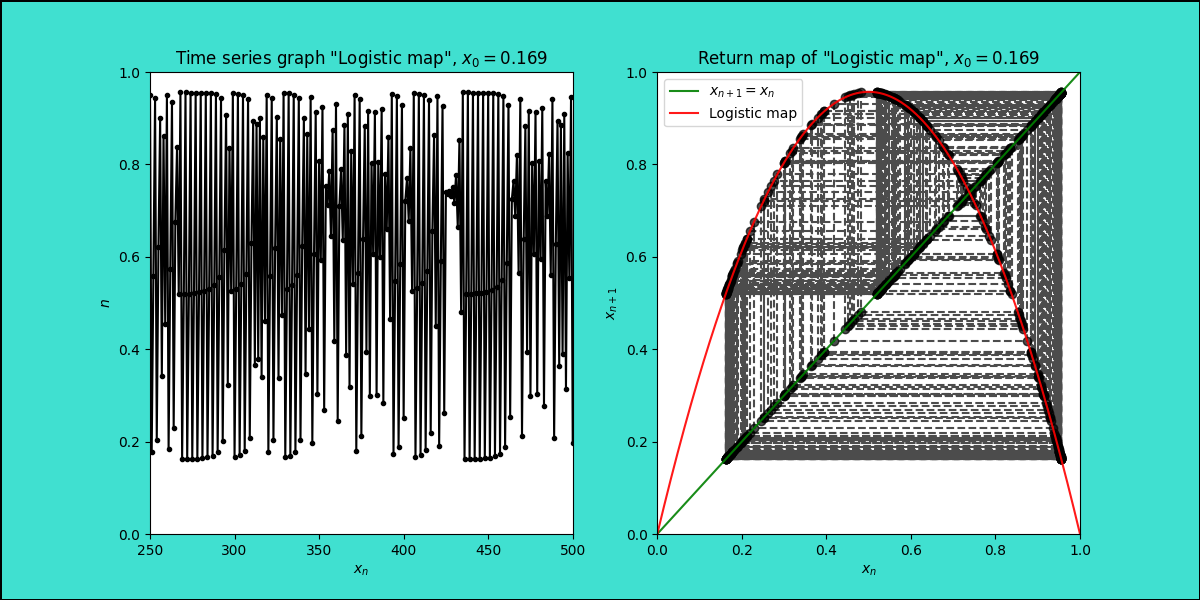
\includegraphics[keepaspectratio, scale=0.5]{images/Problem7/tast7_2.png}
\end{figure}
\subsubsection{考察}
課題1と比較すると $r$ の変化は $0.0001$ なのに対し、時系列グラフとリターンマップには大きな変化が見られた。また、初期値をランダムにとっているため複数回プログラムを実行させた結果、毎回違うグラフが出力された。よって、$r = 3.8284$ のときは、カオスの条件に当てはまると考察した。また課題1の $r$ の値から、$r = 3.8284 と r = 3.8285$ の間に周期倍分岐が起きていることが考察できる。

\subsection{課題3}
\subsubsection{問題}
次に説明する写像 $f^{(3)}$ について、リターンマップを描け(横軸$x_n$, 縦軸$x_{n+3}$)\\
 これまで $x_{n+1} = f \left( x_n \right)$ の写像について考えてきた(ここで関数 $f$ は、上で定義したロジスティック写像)。時系列は $x_0, x_1, x_2, x_3, x_4, x_5, ...$ を順に書いてきたが、上のパラメータでは、だいたいの部分において周期3の運動をしている。そこでここでは、3つ飛ばしで時系列とリターンマップを考える。\\
 いま $x_{n+1} = f \left( x_n \right)$ だから、同様に $x_{n+2} = f \left( x_{n+1} \right), x_{n+3} = f \left( x_{n+2} \right)$ が成り立つ。これらをまとめると、$x_{n+3} = f \left( x_{n+2} \right) = f \left( f \left( x_{n+1} \right) \right) = f \left( f \left( f \left( x_n \right) \right) \right)$と書ける。\\
 この、$x_n$ から $x_{n+3}$ を求める式 $x_{n+3} = f \left( f \left( f \left( x_n \right) \right) \right)$ を簡単のために $x_{n+3} = f^{(3)}\left( x_n \right)$ と書くことにする。これまでは、 $x_n$ と $x_{n+1}$ の間のリターンマップを書いてきたが、$x_n$ と $x_{n+1}$ の間のリターンマップを $r = 3.8284$ のときに書いてみよ。また、下右図のようなリターンマップの階段状にはさまれた部分は何を意味するか考えよ。
\subsubsection{画像}
\begin{figure}[htbp]
  \centering
  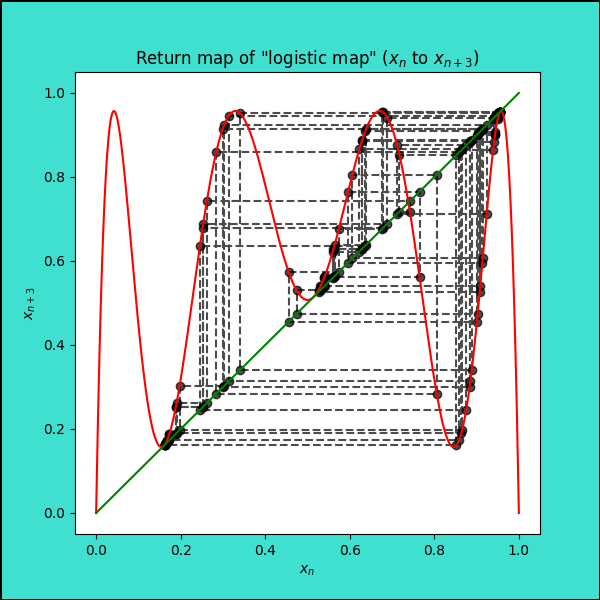
\includegraphics[keepaspectratio, scale=0.5]{images/Problem7/tast7_3.png}
\end{figure}

\subsubsection{考察}
階段上に挟まれた部分はクモの巣図でとっている $x_n$ の時の $x_{n+3}$ の値であると考察した。その理由は範囲が $[0.9561, 0.9565]$ のため曲線の一番右の部分と $x_n = x_{n+3}$ のクモの巣図を拡大しているからである。また、グラフと拡大グラフにより収束したのちに再度発散するような動きになっている。そのため完全には交わっているわけでなく近似していると考察することができる。

\subsubsection{ソースコード}
課題1から課題3までのソースコードを記載している。
\begin{lstlisting}[caption=task7.py]
  from matplotlib import pyplot as plt
  import numpy as np
  from random import uniform


  class Task7():
      def __init__(self) -> None:
          # 初期値 x0 = 0.1
          self.x = uniform(0, 1)
          self.xn = np.linspace(0, 1, 1000)                   # 横軸の範囲と刻み幅
          self.fig = plt.figure(figsize=(12, 6), facecolor='turquoise',
                                linewidth=1, edgecolor='black')

      def logistic(self, r) -> list:
          "リターンマップでのロジスティック写像の座標を持つ配列を返す"
          calc_x = self.x
          x_array = []
          for i in range(1, 501):
              calc_x = r * calc_x * (1 - calc_x)
              if 250 <= i <= 500:
                  x_array.append(calc_x)
          return x_array

      def plot_time_series_graph(self, r: float) -> None:
          "時系列グラフの描画(ロジスティック写像)"
          ax1 = self.fig.add_subplot(1, 2, 1)
          n = list(range(250, 501))
          ax1.plot(n, self.logistic(r), marker='.', color='black')
          ax1.set_title(
              "Time series graph \"Logistic map\", $x_0 = $" + str(round(self.x, 3)))
          ax1.set_xlim(250, 500)
          ax1.set_ylim(0, 1)
          ax1.set_xlabel("$x_n$")
          ax1.set_ylabel("$n$")

      def plot_return_map(self, r) -> None:
          "リターンマップの描画(ロジスティック写像)"
          ax2 = self.fig.add_subplot(1, 2, 2)
          n = self.logistic(r)
          spider_array_x = []                                 # クモの巣図用の配列(x)
          spider_array_y = []                                 # クモの巣図用の配列(y)
          for i in range(1, len(n)):
              spider_array_x.append(n[i - 1])
              spider_array_x.append(n[i])
              spider_array_y.append(n[i])
              spider_array_y.append(n[i])
          logistic_y = []                                     # テント写像のグラフを描くための配列
          for i in self.xn:
              logistic_y.append(r * i * (1 - i))

          ax2.plot(spider_array_x, spider_array_y, marker='o',
                  linestyle='dashed', color='black', alpha=0.7)
          ax2.plot(self.xn, self.xn, color='green',
                  alpha=0.9, label="$x_{n+1} = x_n$")
          ax2.plot(self.xn, logistic_y, color='red',
                  alpha=0.9, label="Logistic map")
          ax2.set_title(
              "Return map of \"Logistic map\", $x_0 = $" + str(round(self.x, 3)))
          ax2.set_xlim(0, 1)
          ax2.set_ylim(0, 1)
          ax2.set_xlabel("$x_n$")
          ax2.set_ylabel("$x_{n+1}$")
          ax2.legend(loc='best')

      def code_problem1(self) -> None:
          r = 3.8285
          self.fig = plt.figure(figsize=(12, 6), facecolor='turquoise',
                                linewidth=1, edgecolor='black')
          self.plot_time_series_graph(r)
          self.plot_return_map(r)
          plt.savefig('複雑系科学演習/Week7/images/task7_1')

      def code_problem2(self) -> None:
          r = 3.8284
          self.fig = plt.figure(figsize=(12, 6), facecolor='turquoise',
                                linewidth=1, edgecolor='black')
          self.plot_time_series_graph(r)
          self.plot_return_map(r)
          plt.savefig('複雑系科学演習/Week7/images/tast7_2')

      def preprocessing(self, x: float) -> float:
          r = 3.8284
          return(r * x * (1 - x))

      def code_problem3(self):
          r = 3.8284
          self.fig = plt.figure(figsize=(6, 6), facecolor='turquoise',
                                linewidth=1, edgecolor='black')

          fff_array_x = []
          fff_array_y = []
          for i in self.xn:
              fff_array_x.append(i)
              fff_array_y.append(self.preprocessing(
                  self.preprocessing(self.preprocessing(i))))

          n = self.logistic(r)
          spider_array_x = []                                 # クモの巣図用の配列(x)
          spider_array_y = []                                 # クモの巣図用の配列(y)
          for i in range(3, len(n), 3):
              spider_array_x.append(n[i - 3])
              spider_array_x.append(n[i])
              spider_array_y.append(n[i])
              spider_array_y.append(n[i])
          plt.plot(spider_array_x, spider_array_y, marker='o',
                  linestyle='dashed', color='black', alpha=0.7)
          plt.plot(fff_array_x, fff_array_y, color='red', label='$Logistic map$')
          plt.plot(self.xn, self.xn, color='green', label='$x_{n+3} = x_n$')
          plt.title('Return map of "logistic map" ($x_n$ to $x_{n+3}$)')
          plt.xlabel('$x_n$')
          plt.ylabel('$x_{n+3}$')
          plt.savefig('複雑系科学演習/Week7/images/tast7_3')


  task = Task7()
  task.code_problem1()
  task.code_problem2()
  task.code_problem3()
\end{lstlisting}

\subsection{課題4}
$x_{n+1} = f \left( x_n \right)$ である時、$x_{n+2} = f \left( x_{n+1} \right), x_{n+3} = f \left( x_{n+2} \right)$ である。従って、$x_{n+3} = f \left( f \left( x_{n+1} \right) \right) = f \left( f \left( f \left( x_n \right) \right) \right)$と書ける。$y = f \left( f \left( f \left( x_n \right) \right) \right)$ のグラフを描き、この曲線が $y = x$ と区間 $[0, 1]$ において互いに異なる3つの点で接する時の $r$ の値は、$r = 1 + \sqrt{8}$ であることをグラフを描いて確認せよ。
\subsubsection{画像}
\begin{figure}[htbp]
  \centering
  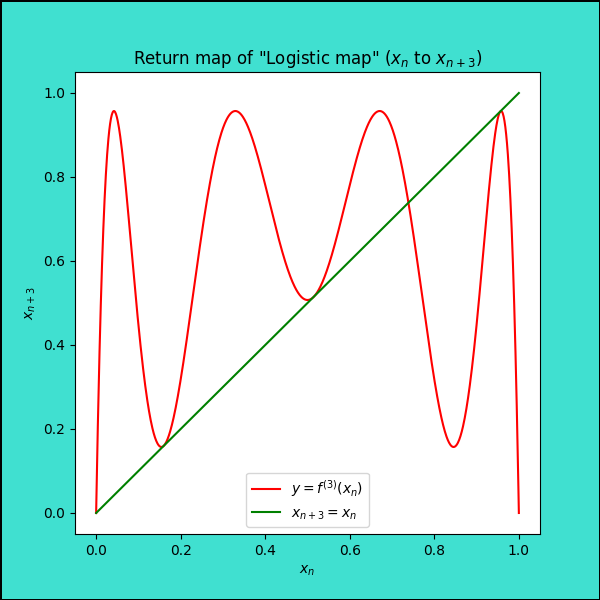
\includegraphics[keepaspectratio, scale=0.5]{images/Problem7/tast7_4.png}
\end{figure}

\subsubsection{考察}
画像から、$r = 1 + \sqrt{8} のとき y = f^{(3)} \left( x_n \right) と x_{n+1} = x_n$ は3点で接していると確認することができる。また、課題3の挟まれた部分のグラフを見ると、$r = 3.8284$ のときには$y = f^{(3)} \left( x_n \right) と x_{n+1} = x_n$ は接することなく収束したのち発散していることが読み取れる。さらに、$1 + \sqrt{8} = 3.82842712474...$ である。以上のことから、$r = 1 + \sqrt{8}$ を境に3周期の特徴を持つと考察することができる。

\subsubsection{ソースコード}
\begin{lstlisting}[caption=task7-4.py]
  from matplotlib import pyplot as plt
  import numpy as np
  from random import uniform


  class Week7Task4():
      def __init__(self) -> None:
          self.x = uniform(0, 1)
          self.r = 1 + 8**(1 / 2)
          self.xn = np.linspace(0, 1, 1000)
          self.fig = plt.figure(figsize=(6, 6), facecolor='turquoise',
                                linewidth=1, edgecolor='black')

      def preprocessing(self, x: float) -> float:
          """前処理"""
          return(self.r * x * (1 - x))

      def code_problem4(self):
          """r = 1 + √8のときのグラフ"""

          fff_array_x = []
          fff_array_y = []
          for i in self.xn:
              fff_array_x.append(i)
              fff_array_y.append(self.preprocessing(
                  self.preprocessing(self.preprocessing(i))))
          plt.plot(fff_array_x, fff_array_y, color='red',
                  label='$y = f^{(3)}(x_n)$')
          plt.plot(self.xn, self.xn, color='green', label='$x_{n+3} = x_n$')
          plt.title('Return map of "Logistic map" ($x_n$ to $x_{n+3}$)')
          plt.xlabel('$x_n$')
          plt.ylabel('$x_{n+3}$')
          plt.legend(loc='best')
          plt.savefig('複雑系科学演習/Week7/images/tast7_4')


  task = Week7Task4()
  task.code_problem4()
\end{lstlisting}

\subsection{課題5}
\subsubsection{問題}
4の結果から $r$ の値が $r = 1 + \sqrt{8}$ より大きい場合と小さい場合において、$x_{n+1} = f \left( x_n \right)$ の安定固定点が幾つあるか理由を述べて答えよ。
\subsubsection{考察}
前回のレポート課題3であるロジスティック写像の分岐図を見て考察した。その結果、$r > 1 + \sqrt{8}$ の場合は3周期をもつときとカオスの状態のときの2つの場合があることが読み取れる。具体的には、$r = 1 + \sqrt{8}$ から進むにつれ周期倍分岐を起こし、その後カオスの状態へと変化していく。よって、安定固定点は$3, 6, ...$ と変化していくと考察した。また、$r < 1 + \sqrt{8}$ の場合は、カオスの状態になるため安定固定点はないと考察した。

\subsection{課題6}
\subsubsection{問題}
4,5から $r = 1 + \sqrt{8}$ の場合に生じたラミナーとバーストは$x_{n+3} = f \left( f \left( f \left( x_n \right) \right) \right)$ の値と $x_n$ の値がどのように変化する時に現れる現象であるか説明せよ。
\subsubsection{考察}
複数回実行するとラミナーとバーストの周期性は捉えることができなかった。
